\chapter{Background}\label{cha:background}

Maze has a long history spanning thousands of years. It intrigued the ancient philosophers, artists, and scientists. In the modern days, we can easily say that mazes are everywhere.
From child puzzles traced by finger to psychology experiments on mice in a laboratory to well-known Pac man games or even the movie Labyrinth from 1986. But the omnipresence of mazes is even greater. 
The mathematicians were also intrigued by mazes and are still studying them carefully. It was very soon noticed that the maze construction may also be presented as a graph. Every problem which may be presented as a graph problem is subject to the same laws as the labyrinth. And so we can discover an enormous variety of real-life applications of maze theory such as navigation systems, transportation route planning systems, building complexity in video games, and solving networking and electrical problems.
As by its popularity, it can be stated with ease that studying the maze generating and solving algorithms, searching for difficulty measures, and searching for a new better solution for many different real-life applications is important, both for amateurs, specialists, and society.  In this chapter, I provide a theoretical background of maze generating algorithms, maze solving algorithms, and other theoretical concepts from the graph theory required to better understand the problems included in this paper. I will also present a background of determining the difficulty of a maze. 

\section{Theoretical Graph Theory Background}\label{sec:theoreticalBackground}
In the following section I will discuss the most important mathematical conepts from graph theory, and i will establish a naming convetion to follow in this paper. 
\begin{definition}
	A set is an object of distinct elements where no element is a set itself. 
\end{definition}
\begin{definition}
A graph according to Trudeau's definition \cite{1}, it's an \textit{object consisting of two sets called vertex set and edge set}. The vertex set is a finite, nonempty set and the edge set may be empty. A graph usually denoted as $ G = (V, E)$ is a pair of a $V$ set of nodes (\textit{vertices}), and $E$ set of (\textit{edges}).\cite{2}. 
 \end{definition}
In this paper, I will consider three interesting subgroups of graphs.
 \begin{itemize}
 \item[$-$] Weighted graph
 \item[$-$] Directed graph
 \item[$-$] Cyclic graph
 \end{itemize}
 \begin{figure}
	\centering
	\begin{subfigure}{.5\textwidth}
	  \centering
	  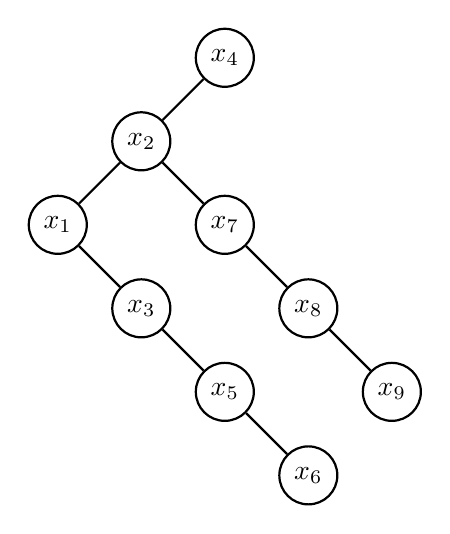
\begin{tikzpicture}[node distance={15mm}, thick, main/.style = {draw, circle}] 
		\node[main] (1) {$x_1$}; 
		\node[main] (2) [above right of=1] {$x_2$}; 
		\node[main] (3) [below right of=1] {$x_3$}; 
		\node[main] (4) [above right of=2] {$x_4$}; 
		\node[main] (5) [below right of=3] {$x_5$}; 
		\node[main] (6) [below right of=5] {$x_6$}; 
		\node[main] (7) [below right of= 2] {$x_7$};
		\node[main] (8) [below right of= 7] {$x_8$};
		\node[main] (9) [below right of= 8] {$x_9$};
		\draw (1) -- (2);
		\draw (2) -- (4);
		\draw (1) -- (3);
		\draw (3) -- (5);
		\draw (5) -- (6);
		\draw (2) -- (7);
		\draw (7) -- (8);
		\draw (8) -- (9);
		\end{tikzpicture} 
	  \caption{An undirected, unweighted, acyclic graph \\ of maze in Figure X}
	  \label{fig:sub1}
	\end{subfigure}%
	\begin{subfigure}{.5\textwidth}
	  \centering
	  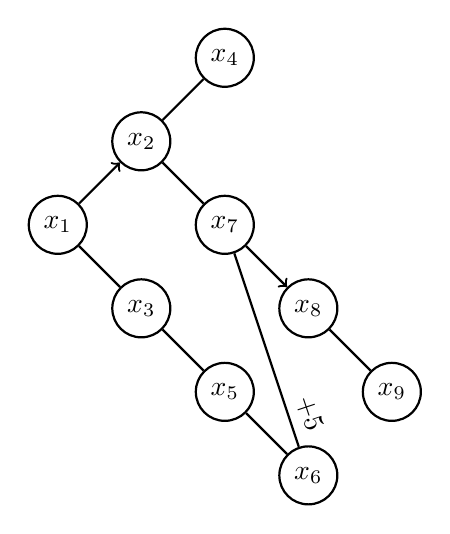
\begin{tikzpicture}[node distance={15mm}, thick, main/.style = {draw, circle}] 
		\node[main] (1) {$x_1$}; 
		\node[main] (2) [above right of=1] {$x_2$}; 
		\node[main] (3) [below right of=1] {$x_3$}; 
		\node[main] (4) [above right of=2] {$x_4$}; 
		\node[main] (5) [below right of=3] {$x_5$}; 
		\node[main] (6) [below right of=5] {$x_6$}; 
		\node[main] (7) [below right of= 2] {$x_7$};
		\node[main] (8) [below right of= 7] {$x_8$};
		\node[main] (9) [below right of= 8] {$x_9$};
		\draw[->] (1) -- (2);
		\draw (2) -- (4);
		\draw (1) -- (3);
		\draw (3) -- (5);
		\draw (5) -- (6);
		\draw (2) -- (7);
		\draw (6) -- node[midway, above left, sloped, pos=0] {+5} (7);
		\draw[->] (7) -- (8);
		\draw (8) -- (9);
		\end{tikzpicture} 
	  \caption{A directed, weighted graph with cycle of maze in Figure Z}
	  \label{fig:sub2}
	\end{subfigure}
	\caption{A figure with two subfigures}
	\label{fig:test}
	\end{figure}

Applying \textit{weight} or \textit{direction} to edges. We are receiving a \textit{ weighted graph} or \textit{directed graph}. A cyclic graph consists of at least one single \textit{cycle}, which means at least 3 vertices connect with each other in a closed chain. 

\begin{definition}
An Adjacency Matrix of a graph $G=(V, E)$ is a representation in which the vertices are numbered in some arbitrary way eg. $1,2,3,\dots, |V|$. The representation of a Matrix of
consisting $|V|x|V|$ such that: 
$$A(i,j)=\begin{cases}
1, if (i,j)\in E,\\
0, otherwise\\
\end{cases}$$
Figures 22.1(c) and 22.2(c) are the adjacency matrices of the undirected and directed graphs respectively.
The adjacency matrix of a graph requires $\varTheta(V^2)$memory, independent of the number of edges in the graph.
\end{definition}
\begin{figure}
	\centering
	\begin{subfigure}{.5\textwidth}
	  \centering
	  $\begin{pmatrix}
		0&1&1&0&0&0&0&0&0\\
		1&0&0&1&0&0&1&0&0\\
		1&0&0&0&1&0&0&0&0\\
		0&1&0&0&0&0&0&0&0\\
		0&0&1&0&0&1&0&0&0\\
		0&0&0&0&1&0&0&0&0\\
		0&1&0&0&0&0&0&1&0\\
		0&0&0&0&0&0&1&0&1\\
		0&0&0&0&0&0&0&1&0\\
	\end{pmatrix}$
	  \caption{An adjacency matrix of a  undirected, unweighted, \\acyclic maze}
	  \label{fig:sub1}
	\end{subfigure}%
	\begin{subfigure}{.5\textwidth}
	  \centering
	  $\begin{pmatrix}
		0&1&1&0&0&0&0&0&0\\
		0&0&0&1&0&0&1&0&0\\
		1&0&0&0&1&0&0&0&0\\
		0&1&0&0&0&0&0&0&0\\
		0&0&1&0&0&1&0&0&0\\
		0&0&0&0&1&0&5&0&0\\
		0&1&0&0&0&0&0&1&0\\
		0&0&0&0&0&0&0&0&1\\
		0&0&0&0&0&0&0&1&0\\
	\end{pmatrix}$
	  \caption{An adjacency matrux of a weighted, directed, cyclic maze}
	  \label{fig:sub2}
	\end{subfigure}
	\caption{Examples of different adjacency matrices}
	\label{fig:test}
	\end{figure}
	\newpage
	\begin{definition}
	A graph in which all vertices are adjacent to all others is said to be complete. 
	\end{definition}
	\begin{definition}
	A density of a graph defines how complete the graph is. The density is defined as the number of edges divided by the number possible. Number possible is a the maximum number of edges that the graph can contain.
	If self-loops are excluded, then the number possible is:\\
	\begin{equation}\label{acyclic_density}
	\frac{n(n-1)}{2}
	\end{equation}
	\begin{eqwhere}
		$n$ is a number of vertices in a graph.\\
	\end{eqwhere}
	If self-loops are allowed, then the number possible is:
	\begin{equation}\label{cyclic_density}
		\frac{n(n+1)}{2}
		\end{equation}
		\begin{eqwhere}
			$n$ is a number of vertices in a graph.
		\end{eqwhere}
		
	\end{definition}
\begin{definition}
A free tree is an undirected, acyclic, connected graph. Let $G = (V,E)$ be an undirected graph. The following properties of a tree apply \\
\begin{itemize}
	\item[$-$] \textit{G} is a free tree,
	\item[$-$] each two nodes in \textit{G} are connected by a unique path,
	\item[$-$] \textit{G} is connected, but if any edge is removed from \textit{E},the graph becomes disconnected,
	\item[$-$] \textit{G} is connected, and $|E| = |V| - 1$,
	\item[$-$] \textit{G} is acyclic, and $|E| = |V| - 1$
	\item[$-$] \textit{G} is acyclic, but if any edge is added to \textit{E}, the graph contains a cycle. 
	\end{itemize}
\end{definition}
\begin{definition}
A binary tree is a tree in which each node has no more than two subordinate nodes. Is composed of three disjoint sets of nodes: a root node, a binary tree called its left subtree, and a binary tree called its right subtree.
\end{definition}
\begin{definition}
A spanning tree \textit{T} is an acyclic tree which connects all the vertices in the graph \textit{G}. The minimum-spanning problem is a problem of determining the tree \textit{T} whose total weight is minimized.
\end{definition}
\begin{definition}
A path in a graph $G$ is a sequence of nodes $v_1, v_2,\ldots,v_k$. The shortest path is a path with the lowest cost between any two given nodes.
\end{definition}
\begin{definition}
A shortest path problem is finding for a given graph $G = (V,E)$, a shortest path from \textit{u} to \textit{v}. Shortest-paths algorithms typically rely on the property that a shortest path be- tween two vertices contain other shortest paths within it.
The shortest path cannot contain any cycles.\cite{introduction }
\end{definition}
\begin{definition}
A cell is a single node in maze matrix. The position of a cell will be given by it's id eg. for a cell with a position $a_{11}$ in a grid, the id will be noted as $"1\char"0023 1"$;	
\end{definition}
\begin{definition}
A degree of a vertex is denoted as $d(v)$ and it describes the number of adjacent cells.\cite{ReHofs}
\end{definition}
\begin{definition}
	An average degree $\bar{d}$for a given graph is given by\cite{ReHofs}:
	\begin{equation}
	\bar{d} = \frac{density}{n-1}	
	\end{equation}
	\textbf{Where:}\\
$n$ & is a number of nodes in the graph\\	
	\end{definition}
\begin{definition}
A dead end is defined as a node with a degree $d(v) = 1$ in the maze that is linked to only one adjacent node.
\end{definition}
\begin{definition}
A fork is defined as a node with a degree $d(v) = 2$ in the maze that is linked to two adjacent nodes.
\end{definition}
\begin{definition}
An intersection is defined as a node with a degree $d(v) = 3$ in the maze that is linked to three adjacent nodes.
\end{definition}
\begin{definition}
A cross id defined as a node with a degree$d(v) = 4$ in the maze that is linked to four adjacent nodes. 	
\end{definition}

\begin{definition}
Cell is smallest element of the maze. The cell keeps the folowning information: it's cooridates, number of neigbours and their's position relative to the cell.	
\end{definition}
\begin{definition}
Grid is considered as a square matrix. It's size defines the size of a maze. The grid keeps information about each cell and their relative positions in a array	
\end{definition}
\begin{definition}
Move is considered as a transition from once cell to one of it's closest neighour. In this paper we are using only NSWE moves. The diagonal moves are forbiden.
\begin{figure}
	\centering
	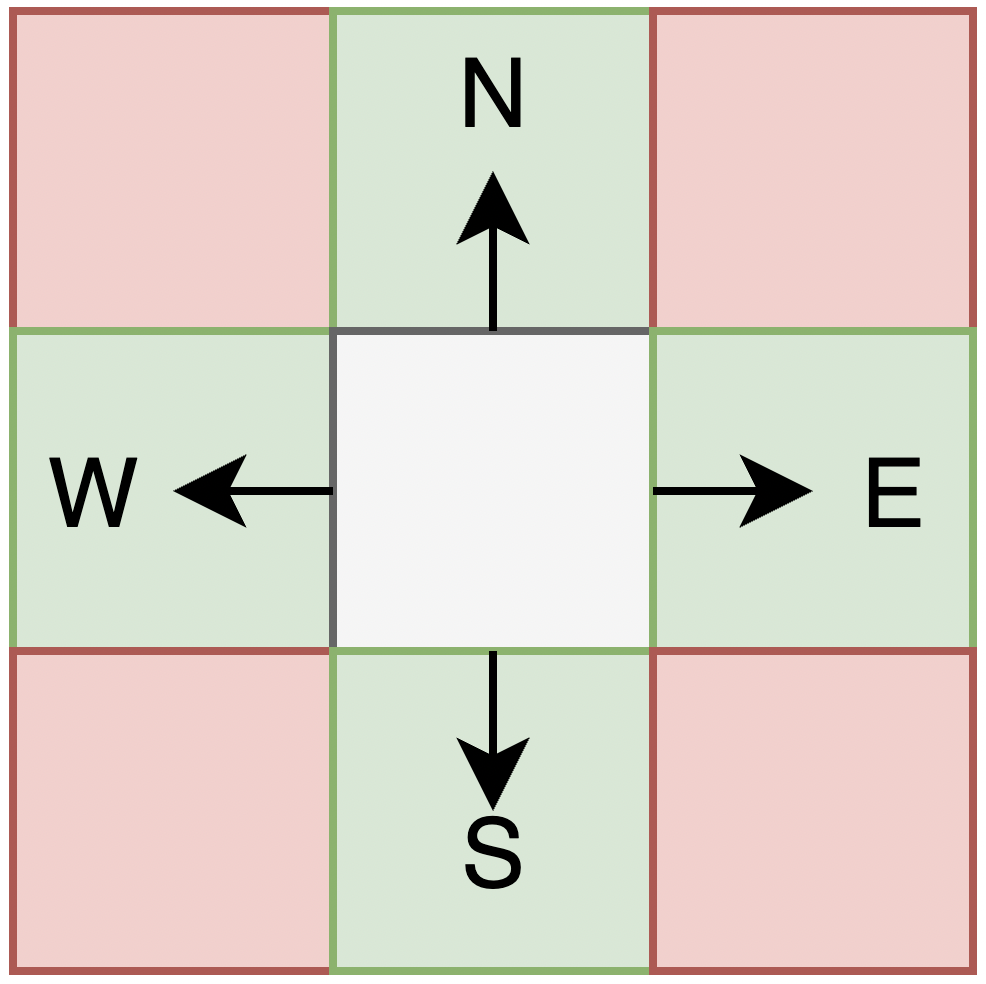
\includegraphics[width=.2\linewidth]{moves}
	\caption{Allowed moves}
\end{figure}		
\end{definition}
\begin{definition}
A maze can be considered as a graph, where each intersection is a vertex, and the path between them is an edge. 
\end{definition}
In this paper, I will be considering only 2D mazes on a rectangular grid [Rys.1]. The grid during the implementation process will be treated as a graph[RysX]. In this paper, I will consider a few types of mazes:
 \begin{itemize}
 \item[$-$] Perfect maze
 \item[$-$] Directed maze
 \item[$-$] Cyclic maze
 \end{itemize}
 The perfect maze will be a maze with only one path between any two given nodes, a directed maze will be a maze with some paths directed in a certain direction, and a cyclic maze will be a maze with at least one cycle. 
 \begin{figure}
	\centering
	\begin{subfigure}{.5\textwidth}
	  \centering
	  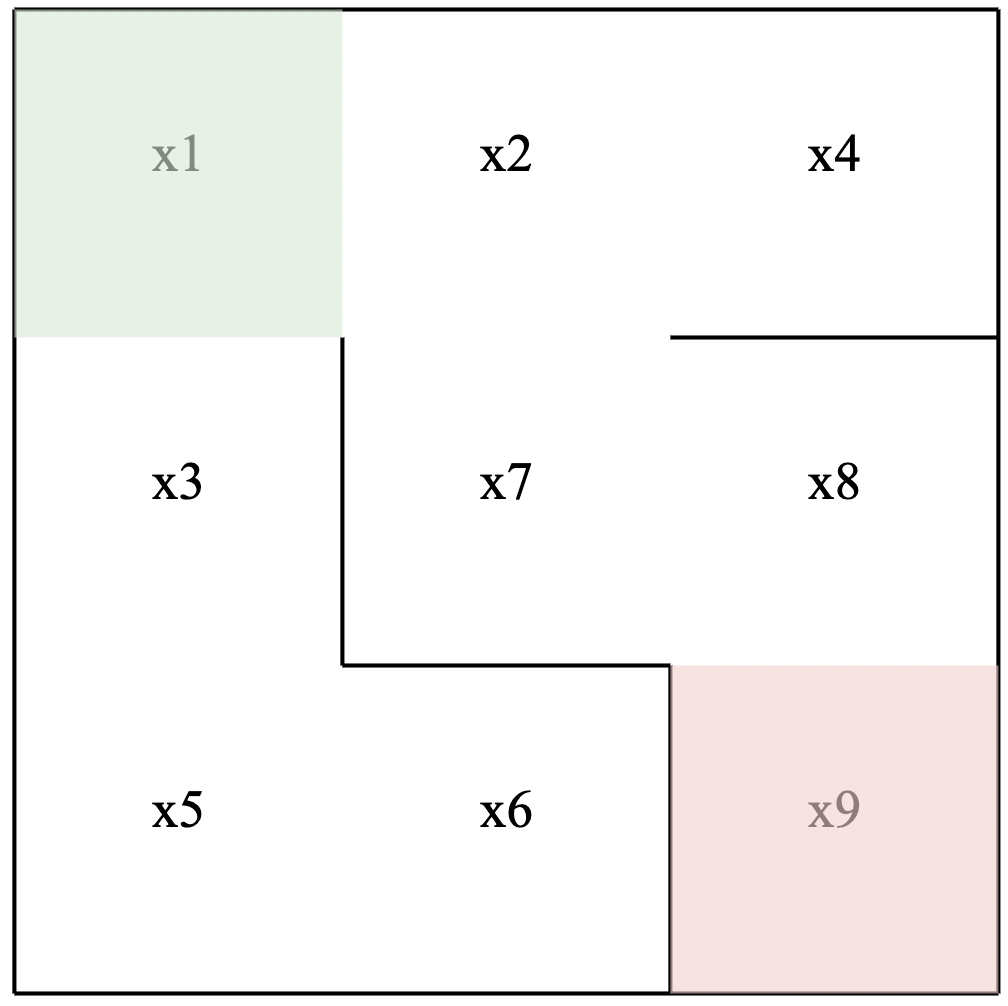
\includegraphics[width=.4\linewidth]{undirected_maze}
	  \caption{An undirected, unweighted, acyclic maze}
	  \label{fig:sub1}
	\end{subfigure}%
	\begin{subfigure}{.5\textwidth}
	  \centering
	  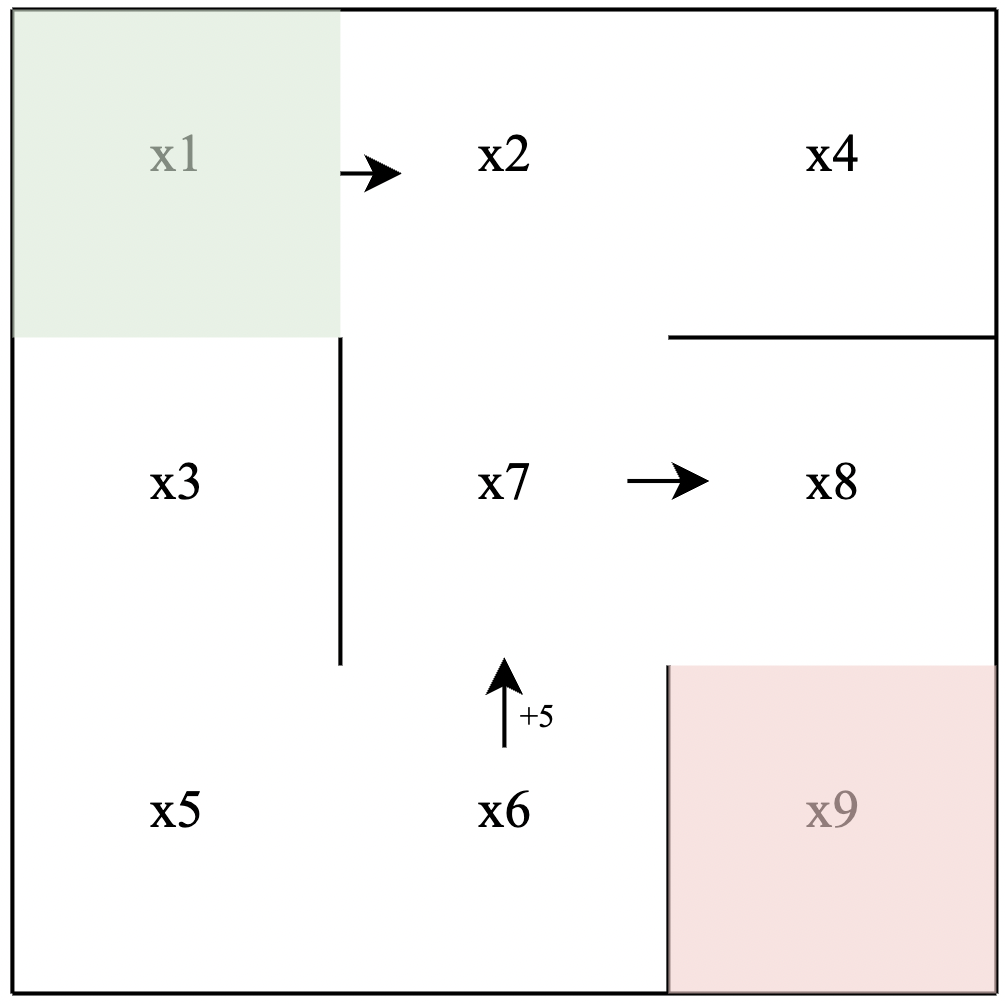
\includegraphics[width=.4\linewidth]{cyclic_maze}
	  \caption{A weighted, directed, cyclic maze}
	  \label{fig:sub2}
	\end{subfigure}
	\caption{Examples of different mazes}
	\label{fig:test}
	\end{figure}
	If not mentioned otherwise, we assume the start and goal position to always be in the upper-left and lower-right, respectively.
 \begin{definition}
A texture is a general term that refers to the style of the passages of a maze, such as how long they tend to be and which direction they tend to go. Some algorithms will tend to produce mazes that all have similar textures.\cite{mazes}
 \end{definition}
 Binary Tree, for example, will always produce mazes with those two unbroken corridors on the north and east.
\begin{definition}
A Canadian traveller problem (CTP) is a problem of finding the shortest path in a given, known graph with changing conditions in it. Objective of this problem is to find best solution in enviroment which is interfered with malicious intension.
\end{definition}
This will be more precisley described in section X.2
\begin{definition}
A Travelling Salesman Problem (TSP) is a problem of finding the shortest bath beetwen given list of nodes int the graph. 
\end{definition}
This will be more precisley described in section X.2
 \section{Maze Generation Algorithms}
\subsection{Binary Tree}
The Binary Tree algorithm is the simplest algorithm for generating a maze. In a given grid, for each cell algorithms decides whether to carve a passage north or east (or any two other directions south/west, south/east etc. ) between two adjacent cells. The algorithm produces a diagonally biased perfect maze which in other words is a random binary tree. For building the whole maze algorithm doesn't require holding the state of the whole grid. The algorithm only looks at one cell at a time. The time complexity for the Binary Tree generator is $O(|V|)$. Below pseudocode for a Binary Tree algorithm.
\begin{lstlisting}[caption={Pseudocode for a Binary Tree Algorithm}]
\begin{algorithm}
\FOREACH cell in the grid
	\STATE let neighbours = [];
	\STATE neighbours.push(cell.north);
	\STATE neighbours.push(cell.east);
	\STATE let index = Math.floor(Math.random() * neighbors.length);
	\STATE let neighbor = neighbors[index];
	\STATE cell.link(neighbor);
\ENDFOREACH	
\end{algorithm}
\end{lstlisting}
\subsection{Aldous-Broder}
The Aldous-Broder is a well-known algorithm to generate uniform spanning trees (USTs) based on random walks. This means that the maze is perfect and unbiased.\cite{4}In a given grid the algorithm randomly chooses any cell, and for this cell randomly chooses a neighbour and if this neighbour wasn't previously visited algorithm links it to the prior cell. Repeat until every cell has been visited. In order to build a spanning tree, the random walk needs to visit every vertex of the graph at least once. The time complexity for the Aldous - Broder generator is $O(|V|^3)$. Below pseudocode for an Aldous- Broder algorithm.
\begin{lstlisting}[caption={Pseudocode for a Aldous-Broder algorithm}]
\begin{algorithm}
\STATE let cell = grid.get_random_cell();
\WHILE unvisited cell in the grid
	\STATE let neighbors = cell.neighbours
	\STATE let index = Math.floor(Math.random() * neighbors.length);
	\STATE let neighbor = neighbors[index];
	\IF neighbour has no links
		\STATE cell.link(neighbor);
	\ENDIF
	\STATE cell = neighbour;
\ENDFOREACH
\end{algorithm}
\end{lstlisting}
\subsection{Recursive Backtracker}
The Recursive Backtracker is one of a Depth First Search algorithm wich may be also used for generationg mazes. It's generates perfect mazes with a very small ratio of dead ends in maze. It's main disadvantage is that it requiers a lot of memory so it's not fast nor efficient. The algorithm starts at randolmy selected cell, and carvs it's way, until it must "turn around" and backtracks to nearest "not carved yet" cell. This process continues until we have discovered all the vertices that are reachable from the original source vertex. The time complexity for Recursive-Backtracker generator is $O(|V|+|E|)$. Below pseudocode for a Recursive-Backtracker algotithm.
\begin{lstlisting}[caption={Pseudocode for a Recursive-Backtracker algorithm}]
	\begin{algorithm}
	\STATE let cell = grid.get_random_cell();
	\STATE let stack = [cell];
	\WHILE stack.lenght > 0
	\STATE let current_cell = stack[stack.lenght - 1];
	\STATE let neighbors = current.neighbors();
		\IF neighbors.length == 0
			\STATE stack.pop()
		\ELSE 
			\STATE let neighbor = neighbors[random]
			\STATE current.make_link(neighbor)
			\STATE stack.push(neighbor)	
	\end{algorithm}
	\end{lstlisting}
\section{Maze Solving Algorithms}
\subsection{Breadth-First Search Algorithm - BFS}
BFS is one of the simplest algorithms for searching a graph. As already mentioned we can consider each maze as a graph so from now on we will call 
BFS a solving algorithm or simply a solver of a given maze. From graph theory, we can state that for a given graph $ G = ( V, E) $, and distinct source 
vertex $s$, BFS explores the edges of $G$ to,,visit' each vertex directly connected with $s$. The algorithm also produces a BFS tree with $s$ root that 
contains all reachable vertexes. The,, shortest path' between $s$ and any vertex $v$ in $G$ is a simple path in the BFS tree, that is, a path containing
the smallest number of edges. \cite{3} ( czy BFS sprawdzi się dla labiryntu o bardzo zachwianej geometrii?)
\subsection{Dijkstra Algorithm}
Dijkstra is a solving algorithm for single-source shortest-path problems. It can be applied on a weighted, directed graph $G=(V, E)$ with a constraint of no negative edges. 
It repeatedly chooses the closest vertex in $V-S$ to add to set S. 
Where \texit{S} is a set of vertices whose final shortest-path weights from the source \textit{s} have already been determined.
As the algorithm floods the graph we say it uses a greedy strategy.
\begin{lstlisting}[caption={Pseudocode for a Dijkstra's algorithm}]
	\begin{algorithm}
	\STATE let distances = new Distances();
	\STATE let frontier = new Array();
	\WHILE unvisited cell in the grid
		\FOREACH linked cell in frontier
			\STATE linked_cell.distance = cell.distance +1;
			\STATE distances.set_cell(linked_cell);
			\STATE frontier.push(linked_cell);
	    \ENDFOREACH
	RETURN distances;
	\end{algorithm}
	\end{lstlisting}
\subsection{A* Algorithm}
$A^*$ algorithm is one of the most path finding algorithm. It uses two fuction, which derives it from the previously described algorithms, which uuses only one function. $A^*$ combines the information that Dijkstra’s Algorithm uses meaning choosing the nodes which are close to the starting point, and implementing new type of information which is heuristic meaning choosing nodes which are estimated to be close to ending point. In the standard terminology used when talking about A*, g(n) represents the exact cost of the path from the starting point to any vertex n, and h(n) represents the heuristic estimated cost from vertex n to the goal. in each loop the algorithm minimize the following function:
\begin{equation}
neighbour.f = neighbour.g + neigbour.h
\end{equation}
\textbf{Where:}
neigbour.g = q.g + distance between q and neighbour\\
is a sum of distances from the starting point to the current node, and the distance from current node to neighbour.	\\
\newline
In maze problems we have a really quick accecs to basic heuristic functions beacouse of a graph implemented as a grid. In this paper We will be using one heuristic method which will be a Manhattan Distance. Beacouse we are using only the NSWE moves in discussed mazes, the Manhattan-Distance is best solution.
Manhatan Distance from neigbour cell to end cellis given as a:
\begin{equation}
neighbour.h = |end\_cell.x - neigbour.x| + |end\_cell.y - neigbour.y|
\end{equation}
\begin{lstlisting}[caption={Pseudocode for a Dijkstra's algorithm}]
	\begin{algorithm}
	\STATE let openlist = new Array();
	\STATE let closelist = new Array();
	\STATE let starcell = maze.startcell;
	\STATE let goalcell = maze.goalcell;
	\STATE starcell.set_g_score();
	\STATE startcell.set_f_score();
	\STATE openlist.push(startcell)
	\STATE let finished = false;
	\WHILE (!finished)
		\STATE let currentcell = openlist    
		.find_cell_with_lowest_fvalue();
		\STATE let neighbours = currentcell.get_links();
			\IF currentcell == goalcell
				finished = true;
				closelist.push(currentcell);
			\ELSE 
			\FOREACH neighbour => neigbours	
			\IF inEitherList(openlist, closelist)
				\STATE g_score = calulate_gscore(cell);
				\STATE f_score = calculate_fscore(cell);
				\STATE parent = setParent(cell);
				\STATE openlist.push(cell)
			\ENDIF
			closelist.push(currentcell);
			openlist.remove(currentcell);
	    	\ENDFOREACH
	\end{algorithm}
	\end{lstlisting}



